\documentclass{article}
\usepackage{custom}
\usepackage{shortex}
\usepackage{tikz}
\title{Chatper 4-6 \quad Change of Basis}

\begin{document}

\maketitle
\pagebreak

Let's say you have vector space, $V$, much like we have already discussed, and we have some subspaces:

\bcent    
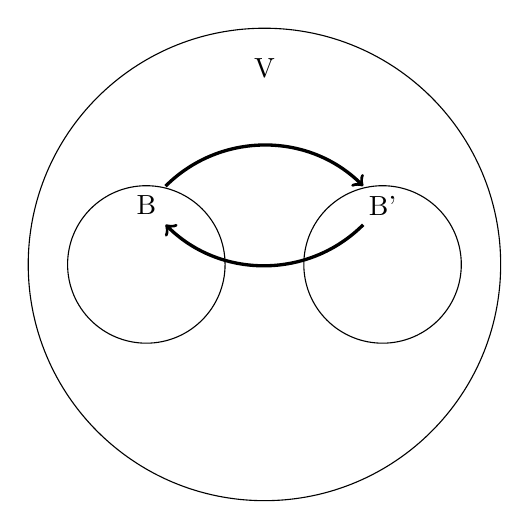
\begin{tikzpicture}[arrow/.style={->, very thick}]
    \draw (0, 0) circle (3);
    \draw (-1.5, 0.0) circle (1);
    \draw (1.5, 0.0) circle (1);

    \node (space) at (0.0, 2.5) {V};
    \node (B) at (-1.5, 0.75) {B};
    \node (B') at (1.5, 0.75) {B'};

    \draw[arrow] (B) to[in=135,out=45] (B');
    \draw[arrow] (B') to[in=-45,out=-135] (B);
\end{tikzpicture}
\ecent

We are given a Matrix, $P$ known as the \textbf{Transition Matrix}. We also with this are guarenteed a inverse $P^{-1}$.

This is useful for many many situations. In any situation where we want to change our "frame of reference" we need to perform this change of basis.

It is like changing what vectors represent and $x, y, \dots$ axes.

\subsection*{Examples}

\[
    B = \cbra{u_{1}, u_{2}} && u_{1} = \begin{bmatrix} 
    1 \\ 0
    \end{bmatrix} \quad& u_{2} = \begin{bmatrix} 
    0 \\ 1
    \end{bmatrix} \\  
    B' = \cbra{u_{1}, u_{2}} && u_{1} = \begin{bmatrix} 
    2 \\ 1
    \end{bmatrix} \quad& u_{2} =\begin{bmatrix} 
    -3 \\ 4 
    \end{bmatrix} \\ 
\]

a)

\[
    P = \begin{bmatrix} 
    B & B'
    \end{bmatrix} = \begin{bmatrix} 
    1 & 0 & 2 & -3 \\ 0 & 1 & 1 & 4
    \end{bmatrix} && P = \begin{bmatrix} 
    2 & -3 \\ 1 & 4
    \end{bmatrix} \\ 
\]

b)

\[
    P^{-1} = \frac{1}{8-(-3)}\begin{bmatrix} 
    4 & 3 \\ -1 & 2
    \end{bmatrix} = \begin{bmatrix} 
    \frac{4}{11} & \frac{3}{11} \\ \frac{-1}{11} & \frac{2}{11}
    \end{bmatrix}
\]

c)

\[
    w &= \begin{bmatrix} 
    3 \\ -5
    \end{bmatrix} \\ 
    \begin{bmatrix} 
    w
    \end{bmatrix}_{B} = Bw &= \begin{bmatrix} 
    1 \\ -5
    \end{bmatrix} \\ 
    \begin{bmatrix} 
    w
    \end{bmatrix}_{B'} = P^{-1}w &= \begin{bmatrix} 
    \frac{-3}{11} \\ \frac{13}{11}
\end{bmatrix}
\]



\end{document}
